%%%%%%%%%%%%%%%%%%%%%%%%%%%%%%%%%%%%%%%%%
% Short Sectioned Assignment
% LaTeX Template
% Version 1.0 (5/5/12)
%
% This template has been downloaded from:
% http://www.LaTeXTemplates.com
%
% Original author:
% Frits Wenneker (http://www.howtotex.com)
%
% License:
% CC BY-NC-SA 3.0 (http://creativecommons.org/licenses/by-nc-sa/3.0/)
%
%%%%%%%%%%%%%%%%%%%%%%%%%%%%%%%%%%%%%%%%%

%----------------------------------------------------------------------------------------
%	PACKAGES AND OTHER DOCUMENT CONFIGURATIONS
%----------------------------------------------------------------------------------------

\documentclass[paper=a4, fontsize=11pt]{scrartcl} % A4 paper and 11pt font size

\usepackage[T1]{fontenc} % Use 8-bit encoding that has 256 glyphs
%\usepackage{fourier} % Use the Adobe Utopia font for the document - comment this line to return to the LaTeX default
\usepackage[english]{babel} % English language/hyphenation
\usepackage{amsmath,amsfonts,amsthm} % Math packages
\usepackage{verbatimbox}
\usepackage{graphicx}
\usepackage{float}


\usepackage{sectsty} % Allows customizing section commands
\allsectionsfont{\centering \normalfont\scshape} % Make all sections centered, the default font and small caps
\usepackage{hyperref}
\usepackage{fancyhdr} % Custom headers and footers
\pagestyle{fancyplain} % Makes all pages in the document conform to the custom headers and footers
\fancyhead{} % No page header - if you want one, create it in the same way as the footers below
\fancyfoot[L]{} % Empty left footer
\fancyfoot[C]{} % Empty center footer
\fancyfoot[R]{\thepage} % Page numbering for right footer
\renewcommand{\headrulewidth}{0pt} % Remove header underlines
\renewcommand{\footrulewidth}{0pt} % Remove footer underlines
\setlength{\headheight}{13.6pt} % Customize the height of the header

\numberwithin{equation}{section} % Number equations within sections (i.e. 1.1, 1.2, 2.1, 2.2 instead of 1, 2, 3, 4)
\numberwithin{figure}{section} % Number figures within sections (i.e. 1.1, 1.2, 2.1, 2.2 instead of 1, 2, 3, 4)
\numberwithin{table}{section} % Number tables within sections (i.e. 1.1, 1.2, 2.1, 2.2 instead of 1, 2, 3, 4)

\setlength\parindent{0pt} % Removes all indentation from paragraphs - comment this line for an assignment with lots of text

\usepackage{verbatimbox}
\usepackage[dvipsnames]{xcolor}

\newcommand{\blau}[1]{{\color{blue}#1}}
\newcommand{\rot}[1]{{\color{WildStrawberry}#1}}
\newcommand{\violet}[1]{{\color{Plum}#1}}
\newcommand{\gruen}[1]{{\color{PineGreen}#1}}
\newcommand{\grau}[1]{{\color{Gray}#1}}
\newcommand{\cn}[1]{\begin{CJK}{UTF8}{gbsn}#1\end{CJK}}

\newcommand{\jl}[1]{\emph{\textbf{Jens: #1}}}
\newcommand{\mg}{\mathcal{G}}
\newcommand{\ten}{\mathcal{T}}
\newcommand{\rl}{\mathbb{R}}

% lecture 2
\newcommand{\shortcode}[1]{\texttt{#1}}
\newcommand*\short[1]{\expandafter\@gobbletwo\number\numexpr#1\relax}
\newcommand{\myheaderbox}[2]{%
	\begin{minipage}[t]{#1}
		\begin{beamerboxesrounded}[upper=block title,lower=block title,shadow=true]%
			{\centering\usebeamerfont*{block title}\rule{0pt}{2.6ex}#2}%
		\end{beamerboxesrounded}\usebeamercolor*{normal text}
	\end{minipage}
}

\newcommand{\mycontentbox}[2]{%
	\begin{minipage}[t]{#1}
		\begin{beamerboxesrounded}[upper=block body,lower=block body,shadow=true]%
			{\centering\usebeamerfont*{block title}\rule{0pt}{2.6ex}#2}%
		\end{beamerboxesrounded}
	\end{minipage}\usebeamercolor*{normal text}
}

\newcommand{\mylcontentbox}[2]{%
	\begin{minipage}[t]{#1}
		\begin{beamerboxesrounded}[upper=block body,lower=block body,shadow=true]%
			{\flushleft\usebeamerfont*{block title}\rule{0pt}{2.6ex}#2}%
		\end{beamerboxesrounded}
	\end{minipage}\usebeamercolor*{normal text}
}

\usepackage{xcolor}
\usepackage{enumitem}
\usepackage{hyperref}
\usepackage{ucs}
\usepackage{listings}
\lstset{basicstyle=\ttfamily\footnotesize,tabsize=2,frame=lines,aboveskip=10pt,belowskip=10pt,captionpos=b,breaklines=true}

\def\changemargin#1#2{\list{}{\rightmargin#2\leftmargin#1}\item[]}
\let\endchangemargin=\endlist 

\setlist[itemize,1]{label={\fontfamily{cmr}\fontencoding{T1}\selectfont$\vartriangleright$}}
\setlist[itemize,2]{label={\fontfamily{cmr}\fontencoding{T1}\color{NavyBlue}\selectfont$\bullet$}}
\setlist[itemize,3]{label={\fontfamily{cmr}\fontencoding{T1}\selectfont\small$\vartriangleright  $}}

\lstset{ %numbers=left, numberstyle=\tiny,
	basicstyle=\ttfamily\small,
	tabsize=2, %keywordstyle=\underbar, stringstyle=\small,
	backgroundcolor=\color[gray]{0.94} } %, framexleftmargin=2pt}
\lstdefinelanguage{SPARQL}
{%showstringspaces=false,
	morestring=[b]",
	% morestring=[s]{>}{<},
	morecomment=[s]{<?}{?>},
	stringstyle=\ttfamily\color{black},
	identifierstyle=\ttfamily\color{black},
	keywordstyle=\ttfamily\color{blue},
	morekeywords={OPTIONAL, SELECT, CONSTRUCT, ASK, DESCRIBE, DISTINCT, WHERE, MINUS, FILTER, BOUND, UNION, LIMIT, OFFSET, COUNT, AS, DATATYPE, ORDER, GROUP, BY, NOT, EXISTS, PREFIX, langMATCHES, LANG, SPARQL}
}
\lstdefinelanguage{SQL}
{%showstringspaces=false,
	morestring=[b]",
	% morestring=[s]{>}{<},
	morecomment=[s]{<?}{?>},
	stringstyle=\ttfamily\color{black},
	identifierstyle=\ttfamily\color{black},
	keywordstyle=\ttfamily\color{blue},
	morekeywords={OPTIONAL, FROM, ON, JOIN, SELECT, CONSTRUCT, ASK, DESCRIBE, DISTINCT, WHERE, MINUS, FILTER, BOUND, UNION, LIMIT, OFFSET, COUNT, AS, DATATYPE, ORDER, GROUP, BY, NOT, EXISTS, PREFIX, langMATCHES, LANG, SPARQL}
}
\lstdefinelanguage{Cypher}
{%showstringspaces=false,
	morestring=[b]",
	% morestring=[s]{>}{<},
	morecomment=[s]{<?}{?>},
	stringstyle=\ttfamily\color{black},
	identifierstyle=\ttfamily\color{black},
	keywordstyle=\ttfamily\color{blue},
	morekeywords={CREATE, OPTIONAL, FROM, ON, JOIN, SELECT, CONSTRUCT, ASK, DESCRIBE, DISTINCT, WHERE, MINUS, FILTER, BOUND, UNION, LIMIT, OFFSET, COUNT, AS, DATATYPE, ORDER, GROUP, BY, NOT, EXISTS, PREFIX, langMATCHES, LANG, SPARQL}
}
\lstset{
	showstringspaces = false,
	emph={SemanticWeb, verlegtBei, titel, Hitzler, Krötzsch, Rudolph, Sure, autor, Buch, Professor, Person, zugehoerigkeit, vorname, Zahl,Projekt,englischerName,franzoesischerName}, emphstyle=\color{black},
	emph={[2]some,only,min,max,and,or,that,not}, emphstyle={[2]\color{blue}},
	aboveskip={0 em},
	belowskip={0 em},
	literate={ö}{{\"o}}1
	{ä}{{\"a}}1
	{ü}{{\"u}}1
}
% Turtle box
\definecolor{olivegreen}{rgb}{0.2,0.8,0.5}
\definecolor{grey}{rgb}{0.5,0.5,0.5}
\lstdefinelanguage{ttl}{
	sensitive=true,
	morecomment=[l][\color{grey}]{@},
	morecomment=[l][\color{olivegreen}]{\#},
	morestring=[b][\color{blue}]\",
	keywordstyle=\color{cyan},
	morekeywords={xmlns,version,owl,rdf,rdfs,xml,xsd}
}

% from 04-SRL.tex
\newcommand{\N}{\mathbb{N}}
\newcommand{\Z}{\mathbb{Z}}
\newcommand{\Q}{\mathbb{Q}}
\newcommand{\R}{\mathbb{R}}
\newcommand{\C}{\mathbb{C}}
\newcommand{\sign}{\operatorname{sign}}
\newcommand{\diag}{\operatorname{diag}}
\newcommand{\Order}{\mathcal{O}}
\newcommand{\Normal}{\mathcal{N}}
\newcommand{\trace}{\operatorname{tr}}
\newcommand{\const}{\mathop{const}}
\newcommand{\Prob}{\mathop{Pr}}
\newcommand{\Expectation}{\mathbb{E}}
\newcommand{\Covariance}{\operatorname{Cov}}
\newcommand{\Risk}{\mathcal{R}}
\newcommand{\continuous}{\mathcal{C}}
\newcommand{\indicator}{\mathbf{1}}
\newcommand{\Span}{\operatorname{span}}
\newcommand{\SV}{\operatorname{SV}}
\newcommand{\Hilbertspace}{\mathcal{H}}
\newcommand{\one}{\boldsymbol{1}}
\newcommand{\scp}[2]{\left\langle #1, #2 \right\rangle}
\newcommand{\dist}{\operatorname{dist}}
\newcommand{\fp}[2]{\frac{\partial #1}{\partial #2}}
\newcommand{\id}{\mathrm{I}}
\newcommand{\ellset}{\{1, \dots, n\}}
\newcommand{\sklearn}{\textit{scikit-learn}}
\newcommand{\code}[1]{\mbox{\texttt{#1}}}

% from 07 Neural Nets
\newcommand{\diagonal}{\operatorname{diag}}

% Markov Networks
\newcommand{\indep}{\operatorname{\,\bot\,}} % statistical independence (multiple symbols used in literature)
\newcommand{\nindep}{\operatorname{\;\not\bot\;}} % statistical independence (multiple symbols used in literature)

%----------------------------------------------------------------------------------------
%	TITLE SECTION
%----------------------------------------------------------------------------------------

\newcommand{\horrule}[1]{\rule{\linewidth}{#1}} % Create horizontal rule command with 1 argument of height
\title{	
\normalfont \normalsize 
\textsc{Faculty of Mathematics, Ruhr University Bochum} \\ [25pt] % Your university, school and/or department name(s)
\horrule{0.5pt} \\[0.4cm] % Thin top horizontal rule
\huge Deep Learning\\{\Large Exercise Sheet 6}\\ % The assignment title
\horrule{2pt} \\[0.5cm] % Thick bottom horizontal rule
}

\author{Asja Fischer} % Your name

\date{\normalsize\today} % Today's date or a custom date

\begin{document}


\maketitle % Print the title
\section{In Class}
\begin{enumerate} 
%\item \textbf{Transfer function}\\
%Consider the sigmoid transfer function
%\begin{align*}
%   \sigma(u) = \frac{1}{1 + e^{-u}} \enspace,
% \end{align*}
% Show that its derivative fulfills
% \begin{align*}
%    \sigma'(u) = \big( 1 - \sigma(u) \big) \cdot \sigma(u) \enspace.
%   \end{align*}


\item \textbf{Feature Matching}\\
(source: Geoffrey Hinton, Coursera)\\
A convolutional neural network is a type of neural network well suited to image recognition. It combines weight sharing with an optimized network topology, that can exploit the 2d-structure of the input data.

We have a convolutional neural network for images of 5 by 5 pixels. In this
network, each hidden unit is connected to a different $4\times4$ region of the
input image:
\begin{itemize}
\item The first hidden unit, $h_1$, is connected to the upper left $4\times4$ portion of the input image (as shown below).
\item The second hidden unit, $h_2$, is connected to the upper right $4\times4$ portion of the input image (as shown below).
\item The third hidden unit, $h_3$, is connected to the lower left $4\times4$ portion of the input image (not shown in the diagram).
\item The forth hidden unir, $h_4$, is connected to the lower right of the $4\times4$ input image (not shown in the diagram).
\end{itemize}
\hspace{2cm}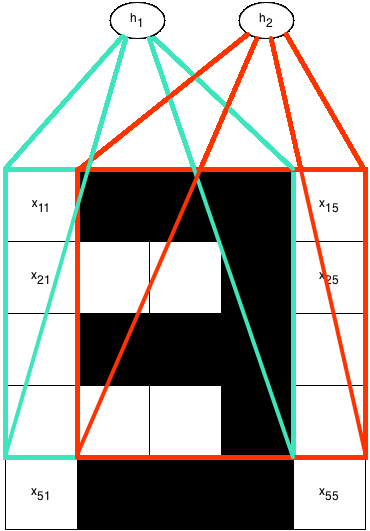
\includegraphics[width=0.3\textwidth]{images/letterE.png}\hspace{2cm}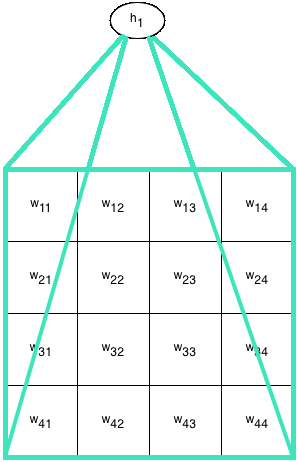
\includegraphics[width=0.3\textwidth]{images/filterF.png}

Because it’s a convolutional network, the weights (connection strengths)
are the same for all hidden units: the only difference between the hidden
units is that each of them connects to a different part of the input image.
In the second diagram, we show the array of weights, which are the same
for each of the four hidden units. For $h_1$, weight $w_{11}$ is connected to the top-left pixel, i.e. $x_{11}$, while for hidden unit $h_2$, weight
$w_{11}$
connects to the pixel that is one to the right of
the top left pixel, i.e.
$x_{12}$. Imagine that for some training case, we have an
input image where each of the black pixels in the top diagram has value 1,
and each of the white ones has value 0. Notice that the image shows a "3"
in pixels.

The network has no biases. The hidden units are linear. The weights of
the network are given as follows:
\begin{align*}
w_{11} &= 1 \;\;\;\; w_{12}=1 \;\;\;\;  w_{13}=1 \;\;\;\; w_{14}= 0 \\
w_{21} &= 0 \;\;\;\; w_{22} = 0 \;\;\;\; w_{23}= 1 \;\;\;\; w_{24}= 0 \\
w_{31} &= 1 \;\;\;\; w_{32}= 1 \;\;\;\; w_{33}= 1 \;\;\;\; w_{34} = 0 \\
 w_{41} &= 0 \;\;\;\; w_{42}=0 \;\;\;\; w_{43}= 1 \;\;\;\; w_{44}= 0
\end{align*}
For the training case with that "3" input image, what is the output
of each of the four hidden units?


\item \textbf{Convolutional Neural Networks}\\
(source: exercise 5-5., exercise sheet 5, Machine Learning, LMU-Munish, Volker Tresp, 2017)\\
In this exercise we address a convolutional neural network (CNN) with one-dimensional input. While two-dimensional CNNs can be used for example for grayscale images, one-dimensional CNNs could be used for
time-series such as temperature or humidity readings. Concepts for the 1D-case are equivalent to 2D networks.
%We interpret data in our network as three-dimensional arrays where a row denotes a feature map, a column denotes a single dimension of the observation, and the depth of the array represents different observations.
%As we will only work with a single input vector, the depth will always be one.
Let the following CNN be given:
\begin{itemize}
\item Input I: Matrix of size $1\times12\times1$. We therefore have an input with twelve dimensions consisting of a single feature map.
\item First convolutional layer with filters $F_0^1=(-1,0,1)$ and
$F_1^1=(1,0,-1)$ that generates two output feature maps from a single input feature map. Use valid mode for convolutions.
\item  Max-pooling layer with stride 2 and filter size 2. Note that max-pooling pools each feature map separately.
\item Convolutional layer with convolutional kernel $F_0^2= ((-1,0,1),(1,0,-1))$ of size $2\times3\times1$.
\item Fully connected layer that maps all inputs to two outputs. The first output is calculated as the negative sum of all its inputs, and the second layer is calculated as the positive sum of all its inputs.
\item Sigmoidal activation function
\end{itemize}
Note, that in this example network we dont have non-linear activation functions after the convolutions for simplicity, but usually one would have.
Calculate the response of the CNN for the following input:
$(0,0,0,0,1,1,1,1,0,0,0,0)$.
\begin{figure}
\center
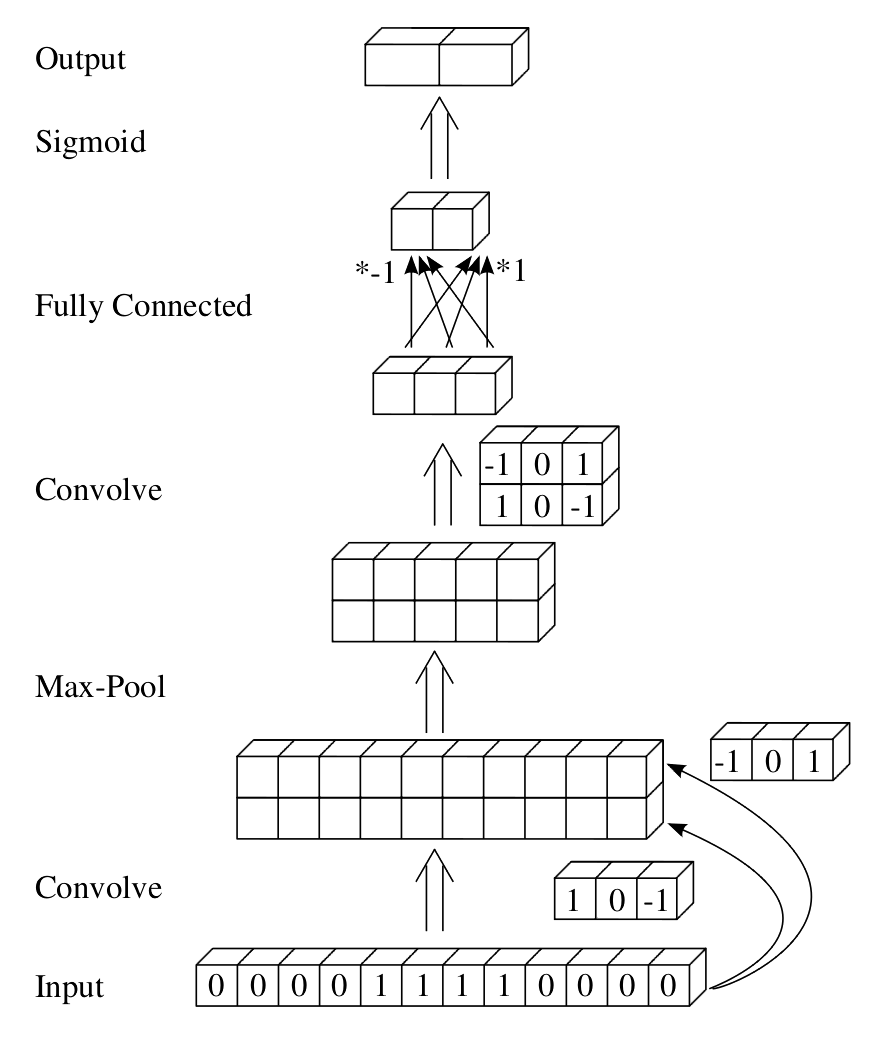
\includegraphics[width=0.6\textwidth]{images/cnn.png}
\end{figure}
\newpage

\item \textbf{Convolution}\\
Let $f$ and $g$ be two discrete, two-dimensional functions.
The \emph{convolution} of $f$ with $g$ is defined by
$$
h(i,j)=(f\ast g)(i,j) =\sum_x\sum_y f(x,y) g(i-x, j-y).
$$

Let us consider the input of the hidden neurons $z_{in, i,j}$  of a convolutional layer (without bias). Let $I$ be the two-dimensional input and, and $W\in\mathbb{R}^{M\times M}$ the corresponding filter, then  
$$
z_{in, i,j}  = \sum_{m=1}^{M} \sum_{n=1}^{M} I_{i+m-1,j+n-1} w_{m,n} \enspace.
$$ 
Interpret this equation in terms of the mathematical definition of a convolution. That is, define $f$ and $g$ such that $z_{in, i,j}=h(i,j)$. 

\end{enumerate}




%\section{At Home}
%\begin{enumerate}
%\item ... some example of actually computing knowledge graph embeddings ...
%\end{enumerate}
\end{document}
